\begin{EXO}{Trois formes d'une fonction du second degré}{}
Soit $f$ la fonction définie sur $\R$ par $ f(x) = 2x^2+4x-16$.
\begin{tcbenumerate}[2]
\tcbitem \tcbitempoint{2} Montrer que pour tout réel $x$, 
\vspace{-0.3cm}\begin{center}$f(x) = 2(x+4)(x-2)$\end{center}
\begin{crep}
$2(x+4)(x-2) $

$= 2(x^2-2x+4x-8 ) $

$= 2x^2+ 4x -16 $

$= f(x)$

\end{crep}

\tcbitem \tcbitempoint{2} Montrer que pour tout réel $x$, 
\vspace{-0.3cm}\begin{center}$f(x) = 2(x+1)^2-18$\end{center}
\begin{crep}
$2(x+1)^2-18 $

$= 2(x^2+2x+1)-18 $

$= 2x^2+4x+2-18 $

$= 2x^2+4x-16= f(x)$ 
\end{crep}
\end{tcbenumerate}
\begin{tcbenumerate}[2][3]
\tcbitem[colframe=black,boxrule=0.4pt,raster multicolumn=2] Choisir la forme la plus adaptée pour répondre aux questions suivantes.
\begin{tcbenumerate}[2][1][alph]
\tcbitem \tcbitempoint{3} Dresser le tableau de variations de $f$
\setrdcrep{seyes=false,correction color=black,correction font=\normalsize}
\begin{crep}[colback=white,colframe=white]%[extra lines=2]
Forme canonique : $f(x) = 2(x+1)^2-18$\\\\

\begin{tikzpicture}
\tkzTabInit{$x$/1,$f$/1.8}
{$-\infty$,$-1$,$+\infty$}
\tkzTabVar{+/$+\infty$,-/$-18$,+/$+\infty$}
\end{tikzpicture}
\end{crep}

\tcbitem \tcbitempoint{1} Résoudre $f(x)=0$

\begin{crep}
Forme factorisée : 

$f(x) = 2(x+1+3)(x+1-3) $

$\phantom{f(x)}= 2(x+4)(x-2)$

$S = \{-4 ; 2\}$
\end{crep}

\tcbitem \tcbitempoint{2} Résoudre $f(x)=-16$

\begin{crep}
Forme développée : $2x^2+4x-16 = -16$

$2x^2+4x = 0 \Rightarrow x(2x+4) = 0$

$S = \{-2 ; 0\}$
\end{crep}

\tcbitem \tcbitempoint{3} Résoudre $f(x)>0$

\begin{crep}
Forme factorisée avec $f(x) = 2(x+4)(x-2)$

$S = \CrochetD-\infty;-4\CrochetG \cup \CrochetD2;+\infty\CrochetG$
\end{crep}
\end{tcbenumerate}
\end{tcbenumerate}

\exocorrection

\begin{tcbenumerate}[2]
\tcbitem \tcbitempoint{2} Montrer que pour tout réel $x$, 
\vspace{-0.3cm}\begin{center}$f(x) = 2(x+4)(x-2)$\end{center}
\begin{crep}
$2(x+4)(x-2) $

$= 2(x^2-2x+4x-8 ) $

$= 2x^2+ 4x -16 $

$= f(x)$

\end{crep}

\tcbitem \tcbitempoint{2} Montrer que pour tout réel $x$, 
\vspace{-0.3cm}\begin{center}$f(x) = 2(x+1)^2-18$\end{center}
\begin{crep}
$2(x+1)^2-18 $

$= 2(x^2+2x+1)-18 $

$= 2x^2+4x+2-18 $

$= 2x^2+4x-16= f(x)$ 
\end{crep}
\end{tcbenumerate}
\begin{tcbenumerate}[2][3]
\tcbitem[colframe=black,boxrule=0.4pt,raster multicolumn=2] Choisir la forme la plus adaptée pour répondre aux questions suivantes.
\begin{tcbenumerate}[2][1][alph]
\tcbitem \tcbitempoint{3} Dresser le tableau de variations de $f$
\setrdcrep{seyes=false,correction color=black,correction font=\normalsize}
\begin{crep}[colback=white,colframe=white]%[extra lines=2]
Forme canonique : $f(x) = 2(x+1)^2-18$\\\\

\begin{tikzpicture}
\tkzTabInit{$x$/1,$f$/1.8}
{$-\infty$,$-1$,$+\infty$}
\tkzTabVar{+/$+\infty$,-/$-18$,+/$+\infty$}
\end{tikzpicture}
\end{crep}

\tcbitem \tcbitempoint{1} Résoudre $f(x)=0$

\begin{crep}
Forme factorisée : 

$f(x) = 2(x+1+3)(x+1-3) $

$\phantom{f(x)}= 2(x+4)(x-2)$

$S = \{-4 ; 2\}$
\end{crep}

\tcbitem \tcbitempoint{2} Résoudre $f(x)=-16$

\begin{crep}
Forme développée : $2x^2+4x-16 = -16$

$2x^2+4x = 0 \Rightarrow x(2x+4) = 0$

$S = \{-2 ; 0\}$
\end{crep}

\tcbitem \tcbitempoint{3} Résoudre $f(x)>0$

\begin{crep}
Forme factorisée avec $f(x) = 2(x+4)(x-2)$

$S = \CrochetD-\infty;-4\CrochetG \cup \CrochetD2;+\infty\CrochetG$
\end{crep}
\end{tcbenumerate}
\end{tcbenumerate}
\end{EXO}